
% to choose your degree
% please un-comment just one of the following
\documentclass[bsc,frontabs,singlespacing,parskip]{infthesis}     % for BSc, BEng etc.
%Readd twoside to make it stick to a side 


% \documentclass[minf,frontabs,twoside,singlespacing,parskip]{infthesis}  % for MInf
\usepackage{hyperref}
\usepackage{todonotes}
\usepackage{cite}
\usepackage{graphicx}
\begin{document}

\title{Inferring Political Opinion From Social Media Data }

\author{Angus Scott}

% to choose your course
% please un-comment just one of the following
\course{Artificial Intelligence and Computer Science}
%\course{Artificial Intelligence and Software Engineering}
%\course{Artificial Intelligence and Mathematics}
%\course{Artificial Intelligence and Psychology }   
%\course{Artificial Intelligence with Psychology }   
%\course{Linguistics and Artificial Intelligence}    
%\course{Computer Science}
%\course{Software Engineering}
%\course{Computer Science and Electronics}    
%\course{Electronics and Software Engineering}    
%\course{Computer Science and Management Science}    
%\course{Computer Science and Mathematics}
%\course{Computer Science and Physics}  
%\course{Computer Science and Statistics}    

% to choose your report type
% please un-comment just one of the following
%\project{Undergraduate Dissertation} % CS&E, E&SE, AI&L
%\project{Undergraduate Thesis} % AI%Psy
\project{4th Year Project Report}

\date{\today}

\abstract{
This is an example of {\tt infthesis} style.
The file {\tt skeleton.tex} generates this document and can be 
used to get a ``skeleton'' for your thesis.
The abstract should summarise your report and fit in the space on the 
first page.
%
You may, of course, use any other software to write your report,
as long as you follow the same style. That means: producing a title
page as given here, and including a table of contents and bibliography.
}

\maketitle
\pagenumbering{roman}

\section*{Acknowledgements}
Insert Acknowledgements here.
\tableofcontents



\chapter{Introduction}
\pagenumbering{arabic}
\todo{introduce what latent attributes are}

\todo{Include detail on why IndyRef is different from american and german elections}

\chapter{Project Outline}
\chapter{Related Work}

\section{Motivation}
The inference of user attributes from social media, particularly with Twitter, has been considered in previous work. Examples typically include the detection of \textit{gender}, \textit{ethinicity}, \textit{brand loyalty}, \textit{regional origin} and \textit{age}.\cite{yahoopaper}\cite{rao2010}

The detection of \textit{Political Affiliation} has also been considered. Most of the research in this area has been focused on one of two political systems. First is the American system, with the 2010 Congressional Midterms\cite{Conover2010predicting}  \cite{politicalpolarisation}\cite{yahoopaper} or the 2012 Presidential Elections \cite{quantpol}. Second is the German system, with the 2009 federal election to the national parliament\cite{predelections}\cite{dividedtheytweet}. 

Typical approaches to the task of classifying a users political persuasion, using social media data, have generally focused around the use of Twitter. There are four main approaches used for classification:

\begin{description}
\item[Profile Features] Features gained directly from a users profile, including: Bio information, usernames, number of followers and location
\item[Tweeting Behaviour] Features that capture how a user tweets, this includes: fraction of retweets, frequency of posting URLs and average number of hashtags
\item[Linguistic Content] Encapsulates the main points of interest/discussion as well as how they use language. Certain keywords may be highly indicative of a particular class, or certain topics of discussion may appear more frequently.
\item[Social Network] Who do users communicate with, you can construct graphical representations where users are a set of nodes and are connected to each other through twitter interactions such as retweets, mentions and follower/following relationships.
\end{description}

This chapter will begin with an introduction to Twitter, and then each of the four approaches will be discussed.

\section{The Twitter Platform}
\label{sec:twitterplatform}
Twitter is a popular microblogging and social network site that allows users to send and read short 140 character messages commonly known as \textit{tweets}. Tweets as used in this report include the 140 character message, along with the associated metadata. This includes features such as: creation dates, user follower counts, coordinates and language. 

As well as tweeting\footnote{Tweeting - The act of broadcasting a tweet} to an audience of \textit{followers}, Twitter users can interact publicly through two main approaches: \textit{retweets} and \textit{mentions}. Retweets often indicate agreement\cite{retweetagreement}, allowing users to rebroadcast content from other users, having the effect of spreading tweets to a larger audience\cite{largeraudiance}. Alternatively, mentions work by allowing someone to refer to a particular Twitter user by including their \texttt{@username} in a tweet, creating a public dialogue between the referrer and referee.

\textit{Hashtags} are another important feature of Twitter, allowing users to tag tweets according to topic and their intended audience. For example \texttt{\#IndyRef} was often used to reference the topic of the Independence Referendum, or \texttt{\#bettertogether} which generally indicated that someone was No Voter or was addressing No Voters.

Twitter has several benefits over other social networking sites \cite{benefitsoftwitter}\cite{quantpol} including:
\begin{enumerate}
\item{Twitter users retweet notable events and participate in the spread of realtime news.}
\item{The 140 character constraint forces tweets to be concise and to the point.}
\item{Users are highly reactionary and discussed events tend to have happened in the recent past.}
\item{Tweets are media rich, and include content like video, image and hyperlinks along with text.} 
\end{enumerate}


\section{Profile Features and Tweeting Behaviour: ``Who you are and how you tweet"}

Most social media services, including Twitter, publicly share information about their users through their site or API such as their usernames, location, short bios, number of friends/followers or tweets/content. This could be used to infer some information about a user such as age of birth, or where the they live, which could all be used to help infer someones political persuasion.


As part of the work done by Rao et al. \cite{rao2010}, they proposed six measures of tweeting behaviour:
\begin{description}
\item[Follower-following Ratio]The ratio between the number of followers a user has and the number of users they are following
\item[Follower Frequency] The number of followers a user has
\item[Following Frequency] The number of users a person is following
\item[Response Frequency] Percentage of tweets from a user that are mentions
\item[Retweet Frequency] Percentage of tweets that are retweets
\item[Tweet Frequency] Percentage of tweets from a user that are not mentions or retweets 
\end{description}

They then compared correlations between these six measures, and four different classification tasks: Age, Gender, Political Orientation and Regional Origin. They found there was no correlation between any of measures and the classes in the different tasks. This would imply that tweeting behaviour have little to no power for classification.

Pennacchiotti and Popescu \cite{yahoopaper} provided a method for obtaining profile features, and another for obtaining tweeting behaviours. They then built two Decision Trees, one for each method, and compared results to other Decision Tree based classifiers described later in this section. 

To obtain profile features, the authors used regular expressions to strip users bio of key information such as gender and age using regular expressions. They also asked a pool of editors to identify ethnicity and gender based on the use of profile pictures. It was found that pictures can be misleading, and that bio fields do not contain enough high quality information to be used directly for classification purposes, and the location field is often to general such as states or countries or contains an imaginary place. 

However, the authors still built a vector of profile based features including: length of username, number of numeric characters and alphanumeric characters in the username, use of avatar picture, number of followers, number of friends, friend/follower ratio, date of account creation, matching patterns from regular expressions and presence in the location field.

To capture tweeting behaviours, the authors built a vector of features including: number of tweets posted by the user, number and fraction of tweets that are retweets, number and fraction of tweets that are mentions, average number of hashtags and URLs per tweet, fraction of tweets that are truncated, average time and std.dev. between tweets, average number and std.dev.of tweets per day, fraction of tweets posted in each of 24 hours.

The two methods performed weakly, with twitter behaviours having an accuracy of 61\%, only 11\% higher than random, which is inline with Rao's work and profile features having an accuracy of 68\%. Profile features may appear to perform well, certainly compared to twitter behaviours, however it performs poorly compared to the 77\% and 86\% obtained with the ensemble of linguistic and network features respectively, which are discussed later in this section. 

In conclusion, profile features and tweeting behaviours are poor measures to use to help classify users political leaning, or many other attributes such as gender and ethnicity. The data they produce is often too noisy and inconsistent to be used for classification purposes, and often don't have any correlation with different classifications at all. Therefore it is best to investigate classification methods based on linguistic and network based features, instead of using statistics of tweeting behaviours and profile features.

\section{Linguistic content: ``What you tweet"}
\label{sec:lingcont}

Tweets contain linguistic information which directly conveys the thoughts and opinions of users. By analysing what the user says/discusses, we can observe similarities between users and from this, group users into different classes. It would be reasonable to assume that users of social media are likely to discuss topics that are of importance/interest to them, and people who share political ideologies/opinions would be likely to discuss similar topics. 

Conover et al. (2010) \cite{Conover2010predicting} propose the use of linear support vector machines (SVMs) to classify 1,000 `highly connected' users into `left' and `right' political classes. The users were manually annotated into `left', `right' and `ambiguous' classes. The tweets were collected over the six weeks preceding the 2010 U.S Midterm Elections. The authors compute accuracy for SVMs built with:
\begin{description}
\item[Full-text] TF-IDF weighted unigrams of tweets (hashtags, mentions, URLs and stop words removed)
\item[Hashtags] Bag of words representation of hashtags in tweets (removed all text that wasn't hashtags and hashtags only used by one user)
\item[Latent Semantic Analysis of Hashtags (LSA)] Applied to the hashtag-user matrix to identify latent factors that correspond to political alignment. 
\end{description}

It was found that the SVM trained on the full-text corpus obtained an accuracy of 79.2\%, but when trained on hashtags the classifier obtained 90.8\%. The addition of LSA to hashtags with the first three dimensions had a minimal improvement on accuracy of 0.1\%, and the addition of subsequent features only decreased performance. 

The paper also makes use of the social network, and is discussed in section \ref{sec:socnet} along with further discussion of what it means to be a `highly connected' user and why the results in this paper may be overly optimistic.

Tumasjan et al. \cite{predelections} is one of the most highly cited of the papers discussed here, and establishes the use of sentiment analysis as a means of detecting political persuasion. The paper uses a corpus of 100,000 tweets referencing the German federal election, collected over the 5 weeks preceding the election. The authors use the LIWC text analysis software and focus on 12 dimensions they feel are relevant to political sentiment: Future orientation, past orientation, positive emotions, negative emotions, sadness, anxiety, anger, tentativeness, certainty, work, achievement, and money.

The paper establishes that the tweets in their corpus were dominated by a small number of users, implying that a  small number of users control the majority of the opinion on Twitter. The authors also establish that candidates who are further from the centre politically have more exaggerated sentiment scores amongst the 12 dimensions mentioned above. The paper concludes by attempting to show that the number of tweets about particular parties reflect the election outcome, and that co-occurrences of two parties reflect real life coalition partners. 

Despite the paper being highly cited, there are two primary criticisms of this paper. First is that tweets were translated from German to English using some machine translation system, and sentiment scores were then calculated from the English translations, even though the LIWC software has a German dictionary. This is likely to introduces a considerable amount of noise, particularly in tweets where slang and incorrect/non-standard grammar is used. Balamurali et al. \cite{balamurali2013lost} found that sentiment analysis performed on translated text performed poorly compared to native text, they attributed this to the failure of the translation system to capture cultural divergence between languages with respect to expressions of sentiment.

The second criticism is the conclusion that number of tweets reasonably reflects the outcome of the election. The authors only compare against one election, and one data point is clearly not enough for any meaningful evaluation. In fact, in the Scottish Referendum corpus, constructed as part of this project, the number of `Yes' leaning tweets exceeds the number of `No' leaning tweets significantly, even though the No Campaign ended up being victorious. 

Pennacchiotti and Popescu \cite{yahoopaper} make use of gradient boosted decision trees (GBDT), combining a collection of weak leaners to form a strong learner. The authors built a balanced corpus of 10,338 self identifying Democrat and Republican voters, with political leanings scrapped from various sources. 

Their weak leaners are a combination of linguistic features and network features, which will be discussed in section \ref{sec:socnet}. The authors use the following linguistic features:

\begin{description}
\item[Prototypical Words] Collection of the 200 most class indicative words per class. Scored by measuring the ratio between the number of occurrences in a class and the number of occurrences in all classes. Similar to Full-Text above, but with less noise.
\item[Prototypical Hashtags] Collection of the 100 most class indicative hashtags per class. Scored by measuring the ratio between the number of occurrences in a class  and the number of occurrences in all classes. Similar to Hashtags above, but with less noise.
\item[Generic Latent Dirichlet Analysis (GLDA)] 100 course grained topics built from corpus of 4 million users. The model is then applied to each test user in order to obtain their topic distribution, which are the features used for classification.
\item[Domain Specific Latent Dirichlet Analysis (DLDA)] Similar to the above, but model is built on users in training set. This produces more fine grained topics that are more class discriminative. 
\item[Sentiment Words] Authors created a small collection of terms $t$ that divide opinions between Republicans and Democrats, and used the tool Opinion Finder 1.5 to find cases where a word carrying sentiment was used with respect to a term in $t$. This was used across all the users tweets, and their scores tallied, to produce a score which indicates your most likely class. 
\end{description}

The authors created a decision tree for each of the features above, and created a function to combine these features together which is a GBDT, an ensemble of the above features. Prototypical Words have an accuracy of 73\%, Prototypical Hashtags 70\%, GLDA 67\%, DLDA 76\%, Sentiment Words 70\% and the ensemble method  with 77\%. 

In conclusion, linguistic data can provide a powerful means of classification, with sentiment scores, topic modelling and prototypical phrases, we can build classifiers that out perform methods that use profile features and tweeting behaviour to classify a users political affiliation. 

\section{Social network: ``Who you tweet"}
\label{sec:socnet}

Many social networks exhibit the concept of homophily - the tendency for users to associate/connect with those who are similar to themselves - and virtual social networks are no exception. As a consequence of this, information about the structure of the network can provide insight, to help infer properties about users that associate with one another, which motivates the use of social networks as a method of user classification.

Conover et al. (2011) \cite{politicalpolarisation} investigates the structure of retweet and user-to-user mention networks. The authors built a corpus of 250,000 tweets over the six weeks leading up to the 2010 U.S congressional midterms. With users given a class label `Republican' or `Democrat'. The authors used a combination of network clustering algorithms, statistical analysis of political tweet content and manually-annotated data. 

Using these tools, the authors found that retweet networks are highly polarised, taking the form of two large clusters of users who distribute content to others in their cluster, with very little overlap between the two clusters. Conversely, it was found that no such structure existed in the user-to-user mention networks, and instead was formed as one large politically heterogenous cluster, where ideologically opposed users interact at a much high rate than in the retweet network. 

The partisan nature of the discourse in retweet networks makes it ideal for the use of classification, hence many of the studies in this area have focused on the use of retweet networks for the purpose of classification.

In addition to their use of linguistic features, Conover et al. (2010) \cite{Conover2010predicting} make use of the social network to classify users. They argue that as many social networks exhibit homophilic properties as described above, they can be used to infer properties about users who tend to associate with one another. The authors form a retweet network composed of the 1,000 most connected users, in other words the 1,000 node subgraph, such that the sum total of the node's connections to the other nodes of the 1,000 node subgraph is maximised.

To classify users the authors used a greedy label propagation method. Each of the 1,000 nodes was given a class 1 or class 2  label using Newman's eigenvector modularity maximisation technique. The algorithm then begins iteratively assigning each node to the class shared by the majority of it's neighbours, and randomly assigning when a tie occurs. This was done until the algorithm converged on a solution. 

The authors found a strong associated between cluster membership and political alignment, and suggested a simple classifier of `Left' if in class 1 or `Right' if in class 2. The method had an accuracy of 95\%, higher than using semantic information. The authors also attempted to combine the two methods by combining cluster assignments and 19 hashtag features selected using Hall's feature selection algorithm and an SVM, but found it performed no better than network clustering alone. 

Whilst the paper provides a solid approach to tackling the problem of detecting political alignment, there is a concern over a biased selection of users for training and testing. By selecting the 1,000 most highly connected users, it is likely that the results are biased, because as Tumasjan et al. \cite{predelections} note, a small number of users dominate the communication in Twitter, and it is very likely that these highly connected users are part of that small group as retweets represent connections, which are observed through communication. Therefore the users who are used for training/evaluation, have an unusually high amount of linguistic content, and connections when compared to most other Twitter users. This leads to the possibility that the results are overly optimistic, if the aim is to use this as a means of classification for general twitter users. 

Pennacchiotti and Popescu \cite{yahoopaper} make use of gradient boosted decision trees (GBDT), combining a collection of weak leaners to form a strong learner. The authors make use of linguistic features (discussed in section \ref{sec:lingcont}) and the following network features:

\begin{description}
\item[Follower Network] Collection of the most exemplar users per class, based on follower relationships. Scored by measuring the ratio between the number of occurrences in a class and the number of occurrences in all classes. Then for each exemplar user in the collection, a boolean feature is set to `1' if a user follows them, and `0' otherwise.

\item[Mention Network] Collection of the 200 most exemplar users per class, based on user-to-user mentions. Scored by measuring the ratio between the number of occurrences in a class and the number of occurrences in all classes. 
\item[Retweet Network] Collection of the 200 most exemplar users per class, based on retweets. Scored by measuring the ratio between the number of occurrences in a class and the number of occurrences in all classes. 
\end{description}
The authors built a decision tree for each of the network features above, and created an ensemble function which is a GBDT, an ensemble of the above features. Follower had an accuracy of 86\%, Mention 68\% and Retweet 66\%.

 It is worth noting that contrary to the work of Conover et al. (2011) \cite{politicalpolarisation}, mentions  have performed better than retweets. This is most likely attributable to the scoring mechanism used in this paper to find prototypical mentions. Mentions may generally be much less polarising, but the scoring still finds terms that maximise the use in one class, but minimise in other classes. So whilst mentions generally may be more heterogenous, the particular mentions selected are still prototypical of a class.

The above paper describes a range of linguistic and network based methods, all of which are weak/reasonable individually, but combine to become a strong classifier with an accuracy of 89\%. 

In conclusion, network based methods for classification can provide excellent means of classification. Retweet networks are politically more partisan than user-to-user mention networks, but does not stop them from an effective means of classification. Follower networks appear to be the best performing networks for classification, this is likely attributable to the fact that you are likely to follow someone because you are interested in what they say, it's a more active form of agreement that simply retweeting something.

\section{Conclusion}

Of the four approaches discussed, it was found that linguistic content and the social network provided the most accurate means of classification, whilst profile features and in particular tweeting behaviour before poorly. However, one issue of note is that for network approaches, the corpuses tend to be a larger or have been select in order to maximise performance by selecting most highly connected users. This approach is therefore unsuitable, or unlikely to yield as positive results as they have done in these studies if they were performed on a smaller corpus. Therefore the work of this thesis has focused on linguistic features, and will be discussed in Chapter \ref{ch:method}.

\chapter{Scottish Indepdendence Referendum Corpus (SIRC)}
\label{ch:corpus}
\section{Introduction}
\section{Scotland Independence Referendum Background}
\label{sec:indybackground}
The Scottish Referendum on Independence was a referendum on Scottish Independence with the intention of establishing Scotland as an independent sovereign state, independent of the rest of the United Kingdom. The election took place on the 18th September 2014, with record turnout of 84.59\% and an electorate of 4,283,392. The referendum concluded with a ``No'' side victory of 55.3\%, over the ``Yes'' side with 44.7\%.

Yes Scotland was the primary campaigning group behind independence, whilst Better Together were campaigning to maintain the union with the rest of the United Kingdom. Many other campaigning groups, including: political parties, businesses, newspapers and famous individuals, were also involved in the campaign. The campaign was widely discussed on social media, with estimates by YouGov stating that 54\% of the electorate got information, regarding the campaign, from social media and other websites. There was much debate during the campaign, on issues including: currencies and monetary policy, public expenditure, EU membership and North Sea oil revenues. 

There was also considered to be several key events on the run-up to the campaign, including The Commonwealth Games that were hosted in Glasgow and the Ryder Cup held at Gleneagles both being hosted in 2014. The year also coincided with the 700 year anniversary of the Battle of Bannockburn, a landmark victory for the Scottish over the English in the First War of Scottish Independence. 


\section{Existing Corpora}
One of the issues of working with Twitter is that under the Twitter API Terms of Service \footnote{\url{https://dev.twitter.com/overview/terms/agreement-and-policy}} you may not share Twitter content, including datasets of tweet text and follower relationships. This therefore makes finding publicly available Twitter corpora very difficult. Because of this, many researchers build their own datasets using the Twitter API or buy them from third party companies such as DataSift \footnote{\url{http://datasift.com}} who pay Twitter to use their data.

Nonetheless, some Corpora exist which have subsequently been taken down, or still remain publicly available because either they have explicit permission from Twitter which allows the creators to keep their datasets available, or Twitter haven't issued or enforced a take down notice. Such examples include the School of Informatics and Computing at Indiana University's ``truthy'' dataset \footnote{\url{http://truthy.indiana.edu/}}, The Edinburgh Twitter Corpus \cite{petrovic2010edinburgh} (which has been made private) and Stanford's SNAP Twitter Dataset \cite{snapnets}. However, due to the time sensitive nature of the task, the truthy and SNAP datasets was not appropriate. However some of the infrastructure that were used as part of the Edinburgh Twitter Corpus were used, and is discussed in Section \ref{sec:construction}. 

Before beginning the process of building my own corpora, I contacted DataSift asking if they would be willing to sponsor a sample of data over the referendum for the project. They very graciously offered to donate a one month sample over the course of the referendum, depending on the details of my project. However this was done in September, when the project was still in the early stages of planning, and there was concerns about how the one month window may not be adequate for some tasks that may have been completed as part of this project. I therefore thanked them and came to the conclusion that the loss in flexibility was too great for a project that was, at that time, in the planning stages. However given the same opportunity again, I would strongly consider working with a data provider, as it provides the opportunity to spend more time modelling and less time mining the data.

\section{Corpus Construction}
\label{sec:construction}

As using a third party corpus wasn't an option, the decision was made to build a corpus for the project. Twitter was used as results would be more comparable with previous work, and the APIs allow for easier access to users published content than the Facebook or Google+ APIs.

The process of building SIRC began by obtaining a collection of politically relevant tweets from the 18th September 2014, the final day of the referendum campaign and the day the vote took place. These tweets were given to me by Miles Osborne who as part of his research and his role in the development of the Edinburgh Twitter Corpus has a cluster of machines dedicated towards Twitter mining. To find the tweets that were relevant to the Scottish referendum, a filter was applied that returned any tweet that matched any one of the tweets in table \ref{tab:hashtagtable}. There were approximately 97,000 tweets returned after this process. 

The hashtags used to find tweets relevant to the referendum were gathered using the hashtagify.me \footnote{\url{http://hashtagify.me/}} tool, which allows you to search for related hashtags given some hashtag. The tool was given the hashtags: \texttt{\#yesscotland} and \texttt{\#bettertogether} and \texttt{\#indyref}, and returned the hashtags given in table \ref{tab:hashtagtable}. It is worth noting that this is a set of temporally non-specific hashtags. Whilst hashtags such as \texttt{\#PatronisingBTlady}\cite{patronisingbtlady} are politically divisive, they have been excluded as they have a short lifespan and were unlikely to be used on the final day of the referendum. 


Of those 97,000 tweets, 1050 users were selected from the collection and given a class label through an annotation procedure described in section \ref{sec:annotate}. Once a user was given an annotation, all of their publicly available tweets (and their associated metadata) that was publicly available and posted between 1st February 2014 and 17th September 2014 were collected using the Twitter API. The users tweets from the 18th September 2014 were then discarded, and the new collection inherited the annotation.

Tweets from the final day of the campaign were used to classify users as they are likely to be the most emblematic of how a user voted, as a user will likely be voting or have already voted once they've tweeted. This choice also minimises the time a user has to change their opinion, and maximises the time a user has to make a decision, as voters generally became less undecided towards the end of the campaign as can be seen in figure \ref{fig:pollingresults}.

\begin{figure}[]
    \centering
    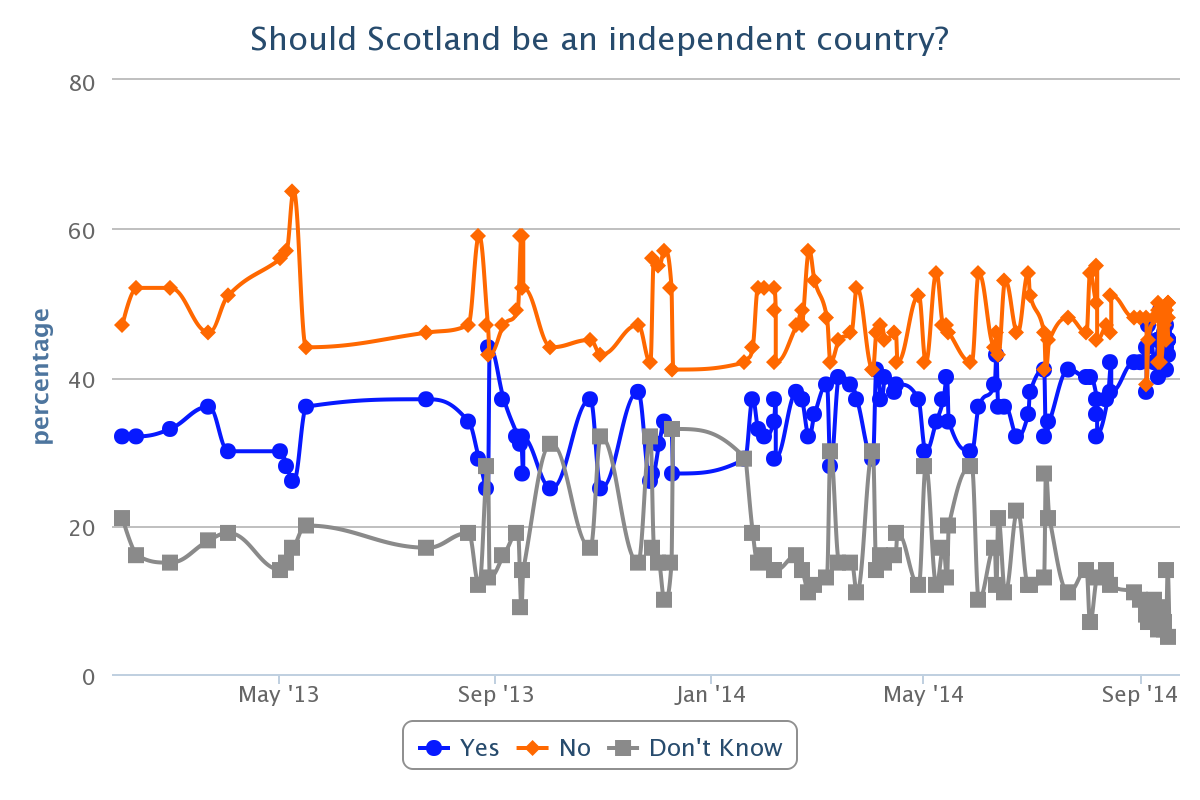
\includegraphics[width=1\textwidth]{pollingresults.png}
    \caption{Aggregation of polling results, where particpants were given the question ``Should Scotland be an independent country?'' created by whatscotlandthinks.org}
    \label{fig:pollingresults}
\end{figure}

\begin{table}
\begin{center}
    \begin{tabular}{ c p{7cm} }
    \hline
    Topic Indicators: & \tt{\#indyref, \#scotland, \#scotdecides, \#scotlanddecides, \#independence} \\ \hline	
     Yes Campaign: & \tt{\#voteyes, \#yesscotland, \#yesscot, \#youyesyet}\\ \hline
     No Campaign: & \tt{\#voteno, \#nothanks, \#bettertogether, \#letsstaytogether} \\ \hline
    Political Parties/Politicians: & \texttt{\#snp, \#labour, \#conservative, \#tory, \#libdem, \#salmond, \#alexsalmond,\#davidcameron, \#gordonbrown, \#alistairdarling}\\
	\hline
   \end{tabular}
\caption{Set of hashtags related to the campaign}
  \label{tab:hashtagtable}
\end{center}
\end{table}

\section{Corpus Annotation and Evaluation}
\label{sec:annotate}
Of those 97,000 tweets, 1050 users were selected from the collection and given a class label of either `y' (most likely to vote yes), `n' (most likely to vote no) or `u' (undeterminable or unrelated) by an annotator familiar with the referendum. They gave the annotation based on the content of the users tweets in the collection.


\section{Corpus Statistics}

Include timeline, most popular hashtags, URLS and mentions
\section{Dataset}
The dataset was collected following the referendum, and is composed of X tweets from Y users, spanning from the 1st February 2014, to 17th September 2014, \todo{Add number of users here} the day prior to the Independence Referendum. The corpus also includes set of user classifications obtained through annotation of  users tweets from the 18th of September.

The first steps in building the corpus, was to obtain tweets from the 18th of September 2014. This first set of tweets were obtained from a Twitter Mining system developed by Sasa Petrovic and Miles Osborne as part of their efforts to create the Edinburgh Twitter Corpus. From this I  was given a collection of tweets that matched a set of hashtags commonly used by users involved in the Yes and No campaigns. 

Hashtags, and their associated campaign are given in Table \ref{tab:hashtagtable}, which were obtained using the hashtagify.me tool. It is worth noting that this is a set of non-event specific hashtags. Whilst hashtags such as \texttt{\#PatronisingBTlady}\cite{patronisingbtlady} are politically divisive, they have been excluded as they have a short lifespan as discussed in Section \ref{sec:twitterplatform}, and are therefore unlikely to be used on the final day of the referendum. 


\todo{Include graph showing strength of hashtag, and how many tweets it appears in }
These tweets are then used as evidence for the annotators to classify a user as Y (Voted Yes in the referendum), N (Voted No in the referendum) or U (Unknown or Undeterminable). We make the assumption that tweets on the final day are the most emblematic of how a user voted, as the opportunity to flip their opinion is minimised andTwitter activity surrounding the event was at it's peak. This is done as there are both technical and ethical issues about obtaining classifications more directly.

After providing a class for each user, we then collect all their publicly available tweets, available from 1st February to 17th September, and their associated meta data using the Twitter API \footnote{Due to a limitation of the Twitter API, you can only collect from the last 3200 published tweets.}. 


\chapter{Methodology}
\label{ch:method}


\section{Dataset}


\section{General approach to user profiling}
\todo{Detail what can be measured in Twitter and how we could use it}
\section{Models}
\todo{Models I plan on implementing, may be moved to eval section}
\subsection{Naive Bayes}
\subsection{Topic Modelling}
\subsection{SVM}
\subsubsection{One class SVMs}
\subsubsection{Alternative SVMs, standard?}
\subsection{Gradient Boosted Decision Trees}
\chapter{Evaluation}
\chapter{Conclusions and Further Work}


% use the following and \cite{} as above if you use BibTeX
% otherwise generate bibtem entries
\bibliography{bibliography}
\bibliographystyle{plain}


\end{document}
